\documentclass{beamer}
\usepackage[utf8]{inputenc}

\usetheme{Madrid}
\usecolortheme{default}
\usepackage{amsmath,amssymb,amsfonts,amsthm}
\usepackage{txfonts}
\usepackage{tkz-euclide}
\usepackage{listings}
\usepackage{adjustbox}
\usepackage{array}
\usepackage{tabularx}
\usepackage{gvv}
\usepackage{lmodern}
\usepackage{circuitikz}
\usepackage{tikz}
\usepackage{graphicx}
\usepackage{gensymb} % For using \degree symbol
\usepackage{enumitem}

\setbeamertemplate{page number in head/foot}[totalframenumber]

% Title Information
\title{4.9.5}
\date{October 9, 2025}
\author{ADHARVAN KSHATHRIYA BOMMAGANI - EE25BTECH11003}

\begin{document}

% Title Slide
\frame{\titlepage}

% Question Slide
\begin{frame}{Question}
Find the equations of the lines that pass through the point $(3,2)$ and make an angle of $40\degree$ with the line $x - 2y = 3$.
\end{frame}

% Step 1: Analyze the Given Line and Point
\begin{frame}{Theoretical Solution}
First, we express the given point and line using column vectors.
\bigskip

The line passes through the point $(3, 2)$. The position vector $\vec{h}$ is:
$$ \vec{h} = \myvec{3 \\ 2} $$
\bigskip

The given line is $x - 2y = 3$. From the formula $\vec{n}^\top \vec{x} = c$, we can identify the \textbf{normal vector} to this line, $\vec{n_1}$:
$$ \vec{n_1} = \myvec{1 \\ -2} $$
\bigskip

The \textbf{direction vector} of the line, $\vec{m_1}$, is orthogonal to its normal vector ($\vec{m_1}^\top \vec{n_1} = 0$). A simple choice is:
$$ \vec{m_1} = \myvec{2 \\ 1} $$
\end{frame}

% Step 2: Finding New Direction Vectors via Rotation
\begin{frame}{Theoretical Solution}
We find the direction vectors, $\vec{m_2}$ and $\vec{m_3}$, for the new lines by rotating $\vec{m_1}$ by $+40\degree$ and $-40\degree$.
\bigskip
The rotation matrix $R(\theta)$ is:
$$ R(\theta) = \begin{pmatrix} \cos\theta & -\sin\theta \\ \sin\theta & \cos\theta \end{pmatrix} $$
\bigskip
\textbf{Rotation by +40\degree}:
\begin{align*}
\vec{m_2} = R(40\degree) \vec{m_1} &= \myvec{2\cos(40\degree) - \sin(40\degree) \\ 2\sin(40\degree) + \cos(40\degree)}
\end{align*}
\textbf{Rotation by -40\degree}:
\begin{align*}
\vec{m_3} = R(-40\degree) \vec{m_1} &= \myvec{2\cos(40\degree) + \sin(40\degree) \\ -2\sin(40\degree) + \cos(40\degree)}
\end{align*}
\end{frame}

% Step 3: Equation of the First Line
\begin{frame}{Theoretical Solution}
To find the equation in normal form $\vec{n}^\top \vec{x} = c$, we need the normal vector $\vec{n_2}$ and the constant $c_2 = \vec{n_2}^\top \vec{h}$.
\bigskip

For a direction vector $\vec{m} = \myvec{u \\ v}$, a normal vector is $\vec{n} = \myvec{-v \\ u}$.
\bigskip

\textbf{Normal Vector $\vec{n_2}$}:
$$ \vec{n_2} = \myvec{-(2\sin(40\degree) + \cos(40\degree)) \\ 2\cos(40\degree) - \sin(40\degree)} $$
\textbf{Constant $c_2$}:
\begin{align*}
c_2 &= \vec{n_2}^\top \vec{h} \\
&= -3(2\sin(40\degree) + \cos(40\degree)) + 2(2\cos(40\degree) - \sin(40\degree)) \\
&= \cos(40\degree) - 8\sin(40\degree)
\end{align*}
\textbf{Equation}: $-(2\sin(40\degree) + \cos(40\degree))x + (2\cos(40\degree) - \sin(40\degree))y = \cos(40\degree) - 8\sin(40\degree)$
\end{frame}

% Step 4: Equation of the Second Line
\begin{frame}{Theoretical Solution}
Similarly, we find the normal vector $\vec{n_3}$ and constant $c_3 = \vec{n_3}^\top \vec{h}$.
\bigskip

\textbf{Normal Vector $\vec{n_3}$}:
$$ \vec{n_3} = \myvec{2\sin(40\degree) - \cos(40\degree) \\ 2\cos(40\degree) + \sin(40\degree)} $$
\bigskip
\textbf{Constant $c_3$}:
\begin{align*}
c_3 &= \vec{n_3}^\top \vec{h} \\
&= 3(2\sin(40\degree) - \cos(40\degree)) + 2(2\cos(40\degree) + \sin(40\degree)) \\
&= \cos(40\degree) + 8\sin(40\degree)
\end{align*}
\textbf{Equation}: $(2\sin(40\degree) - \cos(40\degree))x + (2\cos(40\degree) + \sin(40\degree))y = \cos(40\degree) + 8\sin(40\degree)$
\end{frame}

% Step 5: Figure
\begin{frame}{Plot of the Lines}
\centering
\begin{figure}[h!]
    \centering
    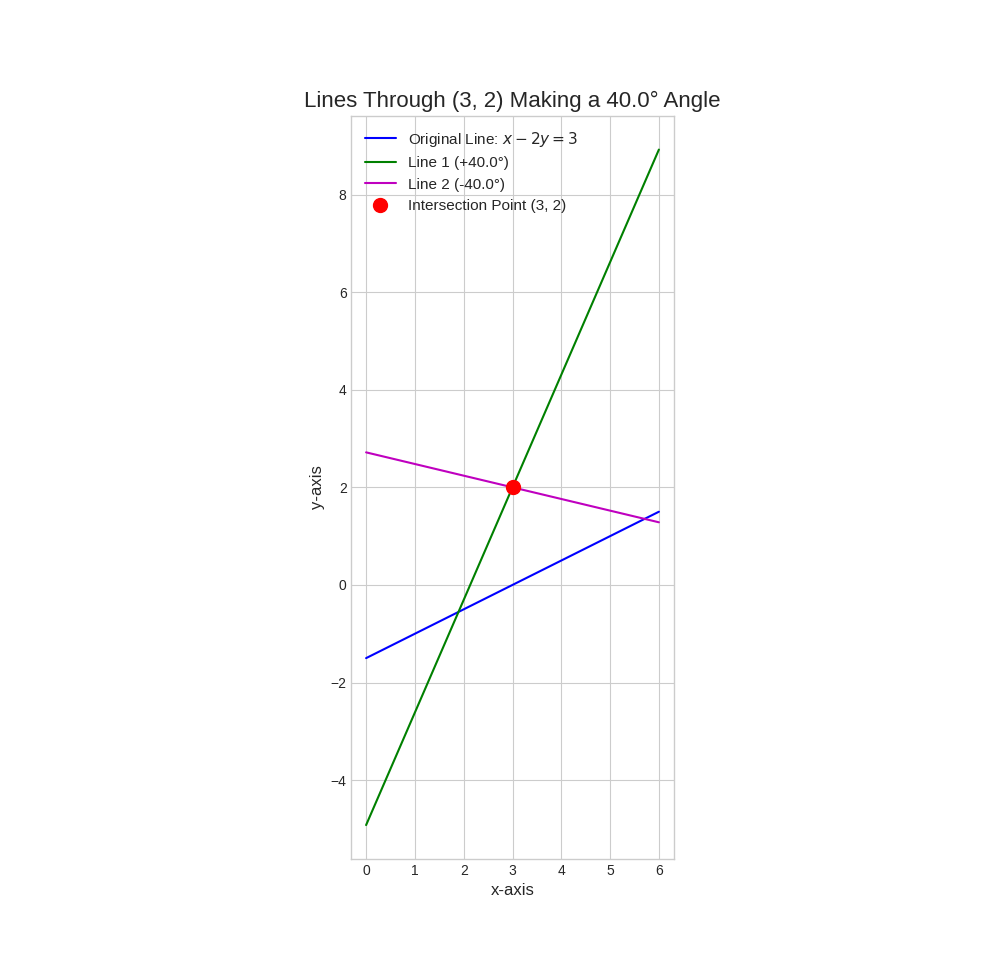
\includegraphics[width=0.7\columnwidth]{figs/fig1.png}
    \caption{Plot showing the original line (blue), the point (3,2), and the two new lines (green and red) making a 40\degree angle with it.}
\end{figure}
\end{frame}

\end{document}+